\documentclass{article}
\usepackage{listings}
\usepackage{tikz}
\usepackage[T1]{fontenc}
\usepackage{graphicx}
\usepackage{systeme}
\usepackage{fixltx2e}
\usepackage{subcaption}
\usepackage{multirow}
\usepackage{amsmath}
\usepackage{amssymb}
\let\emptyset\varnothing
\usepackage{commath}
\lstset{basicstyle=\ttfamily\footnotesize,breaklines=true}
\usepackage{float}

\title{Assignment  3\\ \vspace{0.2cm}

		COMP3670
}



\begin{document}
\setlength\parindent{0pt}
\maketitle
% \newpage
\vspace*{\fill}
    \begin{center}
    
        \textbf{name:}\author{Xuecheng Zhang}
        \\
        \textbf{UID:}u6284513
        
        \vspace{1.8cm}
        
        \date{31/8/2020}
    
    \end{center}
\vspace*{\fill}

\newpage

\textbf{Exercise 1}\\

\textbf{1. Find the gradient $\nabla_\Theta$ $\mathcal{L}_{A,\wedge}(\Theta)$.}\\
\begin{gather}
\mathcal{L}_{A,\wedge}(\Theta) = <y-X\Theta,y-X\Theta>_A + <\Theta,\Theta>_\wedge \notag\\
= (y-X\Theta)^T A (y-X\Theta) + \Theta^T \wedge \Theta \notag \\
= (y^T - \Theta^T X^T )A(y-X\Theta) +  \Theta^T \wedge \Theta \notag \\
= (y^TAy - \Theta^T X^TAy - y^TAX\Theta + \Theta^T X^T A X \Theta) + \Theta^T \wedge \Theta 
\end{gather}

As $y^TAy$ has no element of $\Theta$, the derivative of $y^TAy$ is 0. What is more, using the first identity of computing gradients, we can get $\frac{\partial \Theta^T X^T A y}{\partial \Theta}$ = $(X^TAy)^T$. Using the fourth identity of computing gradients $\frac{\partial x^TBx}{\partial x}= x^T(B+B^T)$, we can get $\frac{\partial  \Theta^T X^T A X \Theta}{\partial \Theta} = \Theta^T(X^T A X + (X^T A X)^T )$ and $\frac{\partial  \Theta^T \wedge \Theta}{\partial \Theta} = \Theta^T (\wedge + \wedge^T )$
\begin{gather}
\nabla_\Theta \mathcal{L}_{A,\wedge}(\Theta) = -(X^TAy)^T - y^TAX + \Theta^T(X^T A X + (X^T A X)^T ) + \Theta^T (\wedge + \wedge^T )\notag \\
= - 2y^TA^TX + \Theta^T(X^T A X + X^T A^T X) + \Theta^T (\wedge + \wedge^T ) \notag \\
= - 2y^TA^TX + 2\Theta^T X^T A X + 2\Theta^T \wedge
\end{gather}
 
2. \textbf{Let $\nabla_\Theta$ $\mathcal{L}_{A,\wedge}(\Theta)$ = \textbf{0}, and solve for \textbf{$\Theta$}}\\
As A, $\wedge$ are symmetric, positive definite so that A = $A^T$, $\wedge^T$ = $\wedge$
\begin{gather}
\nabla_\Theta \mathcal{L}_{A,\wedge}(\Theta) = 0 \notag \\
2y^T A^T X = 2\Theta^T X^T A X + 2\Theta^T\wedge \notag \\
\Theta^T = y^TA^TX(X^T AX + \wedge)^{-1} \notag \\
\Theta = ((X^T AX + \wedge)^{-1})^{T} X^T A y \notag \\
\Theta = ((X^T AX + \wedge)^{T})^{-1} X^T A y \notag \\
\Theta = (X^TAX + \wedge)^{-1} X^T Ay
\end{gather}

3. \textbf{Show that if we choose A = I, and $\wedge$ = $\lambda$I, where $\lambda$ $\in$ R, your answer for 2. agrees with the analytic solution for the standard least squares regression problem with regularization, given by $\Theta = (X^T X + \lambda I)^{-1}X^T y$}.\\

When A = I, and $\wedge$ = $\lambda$I, the $\Theta$ is 
\begin{gather}
\Theta = (X^T I X + \lambda I)^{-1} X^T I y = (X^T X + \lambda I)^{-1}X^T y
\end{gather}

4.\textbf{What advantages are there in choosing $||\Theta||^2_{\wedge}$ over the more standard regularization term $\lambda||\Theta||^2_{2}$?}\\

As $\lambda||\Theta||^2_{2}$ = $\lambda \Theta^T \Theta $ = $\Theta^T \lambda I \Theta$\\
When $\wedge = \lambda I$, $||\Theta||^2_\wedge$ = $\lambda||\Theta||^2_{2}$\\
Therefore,  $\lambda||\Theta||^2_{2}$ is a special case of $||\Theta||^2_\wedge$ which means $||\Theta||^2_\wedge$ can make loss function more generally than standard regularization term $\lambda ||\Theta||_2^2$. \\
Using regular term $\lambda ||\Theta||_2^2$, sometimes it is difficult to find the optimal value $\lambda$, as the result may stuck in local minimal. However, using this $||\Theta||_\wedge^2$ will be more comprehensive because it covers $\lambda ||\Theta||_2^2$ result, and its results will only have better or the same results and not worse than it.\\ 
In this case, we are more likely and easily to find $\wedge$ make the regularisation term not particularly important to the value of loss function, but it limits the weight of $\theta$ and avoids overfitting.\\

\textbf{Exercise 2}\\

1. \textbf{For the $L_2$ loss function, $L_2$($\mu$, D) = $\sum_{i=1}^{N} (\mu - x_i)^2$, show that the optimal choice for $\mu$ is the mean, $\mu = \frac{1}{N} \sum_{i=1}^N x_i$.}\\

Define F($\mu$) = $L_2$($\mu$,D) = $\sum_{i=1}^{N} (\mu - x_i)^2$\\
The smallest loss is obtained when we find $\mu$ which makes the derivative of the loss function to zero.\\
\begin{gather}
\frac{dF(\mu)}{d\mu} = 2(\mu - x_1) + 2(\mu - x_2) + 2(\mu - x_3) + \cdots + 2(\mu - x_N) \notag \\
= 2N\mu - 2(x_1 + x_2 + \cdots + x_N) = 0
\end{gather}
When $2N\mu$ = $2(x_1 + x_2 + \cdots + x_N)$, i.e. $\mu = \frac{x_1 + x_2 + \cdots + x_N}{N} =  \frac{\sum_{i=1}^N x_i}{N}$.\\
When $\mu < \frac{\sum_{i=1}^N x_i}{N}$, $\frac{dF(\mu)}{d\mu}$ <0 indicates that $F(\mu)$ is decreasing to approach to the minimum. When $\mu > \frac{\sum_{i=1}^N x_i}{N} $, $\frac{dF(\mu)}{d\mu}$ >0 indicates that $F(\mu)$ is moving away from the minimum. Therefore, when $\mu$ = $\frac{\sum_{i=1}^N x_i}{N}$ which is mean value of in the set, $F(\mu)$ has the minimum value.\\

\textbf{2. For the $L_1$ loss function, $L_1$($\mu$, D) = $\sum_{i=1}^{N} |\mu - x_i|$, show that the optimal choice for $\mu$ is the median value in the set.}\\

Define $F(\mu)$ = $L_1(\mu,D)$ = $\sum_{i=1}^{N} |\mu - x_i|$ \\

As $\mu$ $\in$ $\mathbb{R}$, the derivative of $F(\mu)$ is:\\

When $\mu$ $\leq$ $x_1$,
\begin{gather}
\frac{dF(\mu)}{d\mu} = \frac{d (x_1 - \mu + x_2 - \mu + \cdots + x_N - \mu)}{d\mu} = -N 
\end{gather}

When $\mu$ $\geq$ $x_n$,
\begin{gather}
\frac{dF(\mu)}{d\mu} = \frac{d(\mu - x_1 + \mu - x_2 + \cdots + \mu - x_N)}{d\mu} = N 
\end{gather}
The minimum value exists among $x_1$ and $x_n$\\

When $x_1$ < $\mu$ < $x_n$,\\
Assume that $x_1$ < $x_j$ < $\mu$ < $x_{j+1}$ < $x_n$, n = 2k, k, j $\in \mathbb{R}$
\begin{gather}
\frac{dF(\mu)}{d\mu} = \frac{d(\mu - x_1 + \mu - x_2 + \cdots + \mu - x_j  + x_{j+1} - \mu + \cdots + x_n - \mu)}{d\mu} \notag \\
= j - (2k -j-1 +1) = 2j - 2k 
\end{gather}
\[
F(\mu) = \begin{cases}
j < k \text{ and } x_j < \mu < x_{j+1} & F(\mu) < 0 \text{. The function is decreasing}\\
j > k  \text{ and }  x_j < \mu < x_{j+1} &  F(\mu) > 0 \text{. The function is increasing}\\
j = k  \text{ and } x_j < \mu < x_{j+1} &  F(\mu) = 0 \text{. The function is constant}
\end{cases}
\]
The function exist minimum value when $x_{\frac{n}{2}} < \mu < x_{\frac{n}{2}+1}$: 
\begin{gather}
\sum_{i=1}^{N} F(\mu) = \mu - x_1 + \mu - x_2 + \cdots + \mu - x_{\frac{n}{2}}  + x_{\frac{n}{2}+1} - \mu + \cdots + x_n - \mu \notag\\ = (\frac{n}{2})\mu - (\frac{n}{2})\mu - \sum_{i=1}^{\frac{n}{2}} x_i + \sum_{i=\frac{n}{2}+1}^{n} x_i = - \sum_{i=1}^{\frac{n}{2}} x_i + \sum_{i=\frac{n}{2}+1}^{n} x_i
\end{gather}
When $ x_{\frac{n}{2}} < \mu < x_{\frac{n}{2}+1}$ have the minimum value $- \sum_{i=1}^{\frac{n}{2}} x_i + \sum_{i=\frac{n}{2}+1}^{n} x_i$\\
The median of the set is $ x_{\frac{n}{2}}$  < $\frac{1}{2}$ ($x_{\frac{n}{2}}$ + $x_{\frac{n}{2}+1}$)< $ x_{\frac{n}{2}+1}$. so when n = 2k, $\mu$ is the median value having the minimum $L_1$ loss value.\\

Assume that $x_1$ < $x_j$ $\leq$ $\mu$ $\leq$ $x_{j+1}$ < $x_n$, n = 2k+1, k, j $\in \mathbb{R}$\\
\begin{gather}
\frac{dF(\mu)}{d\mu} = \frac{d(\mu - x_1 + \mu -x_2 + \cdots + \mu - x_j + x_{j+1} - \mu + \cdots + x_n - \mu)}{d\mu} \notag\\
= j - (n-j) = 2j - (2k + 1) = 2j - 2k -1
\end{gather}

\[
F(\mu) = \begin{cases}
j <= k \text{ and } x_j < \mu < x_{j+1} & F(\mu) < 0 \text{. The function is decreasing}\\
j > k  \text{ and }  x_j < \mu < x_{j+1} &  F(\mu) > 0 \text{. The function is increasing}\\
\end{cases}
\]

When j = k or j = k+1, F($\mu$) have the minimum value since the gradient $\frac{dF(\mu)}{d\mu}$ is approaching to 0. \\

When j = k \begin{gather}
F(x_k) = x_k - x_1 + x_k - x_2 + \cdots + x_k - x_k + x_{k+1} - x_k + \cdots + x_{2k+1} - x_k \notag\\
= x_k - x_1 + x_k - x_2 + \cdots + x_k - x_{k-1} + x_{k+1} - x_k + \cdots + x_{2k+1} - x_k \notag\\
= -2x_k - x_1 - x_2 - \cdots - x_{k-1} + x_{k+1} + x_{k+2} + \cdots + x_{2k+1}
\end{gather}

When j = k + 1 \begin{gather}
F(x_{k+1}) = x_{k+1} - x_1 + x_{k+1} - x_2 + \cdots + x_{k+1} - x_{k} + x_{k+1} - x_{k+1} + \cdots + x_{2k+1} - x_{k+1} \notag\\
= x_{k+1} - x_1 + x_{k+1} - x_2 + \cdots + x_{k+1} - x_{k} + x_{k+2} - x_{k+1} \cdots + x_{2k+1} - x_{k+1} \notag\\
= -x_1 - x_2 -\cdots -x_k + x_{k+2} + x_{k+3} + \cdots x_{2k+1} 
\end{gather} 

\begin{gather}
F(x_{k+1}) - F(x_k) = -x_1 - x_2 -\cdots -x_k + x_{k+2} + x_{k+3} + \cdots + x_{2k+1}  - \notag\\(-2x_k - x_1 - x_2 - \cdots - x_{k-1} + x_{k+1} + x_{k+2}  + \cdots + x_{2k+1}) \\ = x_k - x_{k+1} <0
\end{gather}

Therefore, $F(x_{k+1}) < F(x_{k})$. Thus, when $\mu$ = $x_{k+1}$ = $x_{\frac{1+(2k+1)}{2}}$, n = 2k + 1, $\mu$ is the median value having the minimum $L_1$ loss value. \\
In a conclusion, the optimal choice for $\mu$ is the median value in the set.\\

4. \textbf{For the $L_{\infty}$ loss function, $L_{\infty}$($\mu$, D) = $max_{1 \leq i \leq n}$ $|\mu - x_i|$, show that the optimal choice for $\mu$ is $\frac{x_1+x_n}{2}$,the average of only the largest and smallest data point in the set.}\\

When $\mu$ $\leq$ $x_1$, \\
As $\mu \leq x_1$, the maximum difference between $\mu$ and $x_i$ is when $x_i$ has the max value, which ($x_i$ = $x_n$). 
\begin{gather}
L_{\infty} (\mu,D) = max_{1 \leq i \leq n} |\mu - x_i| = x_n - \mu
\end{gather}
To get the minimum of $L_{\infty} (\mu,D)$, we have to maximize $\mu$. When $\mu$ = $x_1$ we get the minimum value.\\

When $\mu$ $\geq$ $x_n$,\\
As $\mu \geq x_n$, the maximum difference between $\mu$ and $x_i$ is when $x_i$ has the min value, which ($x_i$ = $x_1$).

\begin{gather}
L_{\infty} (\mu,D) = max_{1 \leq i \leq n} |\mu - x_i| = \mu - x_1
\end{gather}
To get the minimum of $L_{\infty} (\mu,D)$, we have to minimize $\mu$. When $\mu$ = $x_n$ we get the minimum value.\\
Above two conditions, we have the minimum $L_{\infty}$($\mu$, D)  = $x_n - x_1$\\

When $x_1 < \mu < x_n$,\\
\textbf{Assume that $\mu$ is closer to $x_1$ than $x_n$ (i.e. $|\mu - x_1|$ < $|\mu - x_n|$)}. Therefore, the maximum of the value is not $|\mu - x_1|$. \\(Situation 1) If there exists $x_k, x_1 < x_k < \mu$ has the maximum distance between $x_k$ and $\mu$. However, it is impossible since the distance between $x_1$ and $\mu$ is farther than the distance between $x_k$ and $\mu$. Also, the maximum of the value is not $|\mu - x_1|$. Therefore, the maximum $x_k$ can only exists between $\mu$ and $x_n$. \\
\begin{figure}[H]
\centering
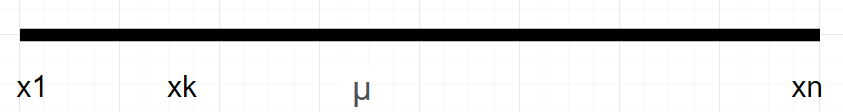
\includegraphics[width = \linewidth]{1.png}
\caption{Situation 1}
\end{figure}
(Situation 2) If there exists $x_k$, $\mu < x_k < x_n$ has the maximum distance between $x_k$ and $\mu$. However, it is impossible since the distance between $x_n$ and $\mu$ is farther than the distance between $x_k$ and $\mu$.
\begin{figure}[H]
\centering
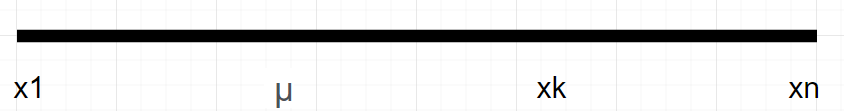
\includegraphics[width = \linewidth]{2.png}
\caption{Situation 2}
\end{figure}


Therefore, when $x_k$ = $x_n$ has the maximum value between $a_k$ and $\mu$. \\
As $F(\mu) = L_{\infty}(\mu,D) = |\mu - x_n| = x_n - \mu$ and $\mu$ is closer to $x_1$, when the distance between $\mu$ and $x_1$ is large but it does not exceed the distance between $\mu$ and $x_n$, $F(\mu)$ is the minimum value. That's when the distance between $\mu$ and $x_1$ is equal to the distance between $\mu$ and $x_n$, i.e. $\mu$ = $\frac{x_1 + x_n}{2}$.\\

\textbf{Assume that $\mu$ is farther to $x_1$ than $x_n$ (i.e. $|\mu - x_1|$ > $|\mu - x_n|$)}.Therefore, the maximum of the value is not $|\mu - x_n|$. \\(Situation 3) If there exists $x_k, \mu < x_k < x_n$ has the maximum distance between $x_k$ and $\mu$. However, it is impossible since the distance between $x_n$ and $\mu$ is farther than the distance between $x_k$ and $\mu$. Also, the maximum of the value is not $|\mu - x_n|$. Therefore, the maximum $x_k$ can only exists between $x_1$ and $\mu$.

\begin{figure}[H]
\centering
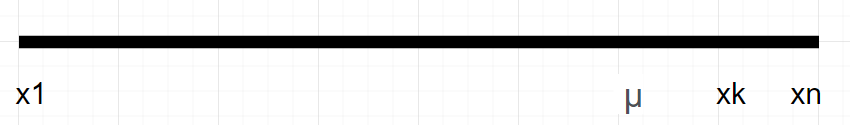
\includegraphics[width = \linewidth]{3.png}
\caption{Situation 3}
\end{figure}
(Situation 4) If there exists $x_k$, $x_1 < x_k < \mu$ has the maximum distance between $x_k$ and $\mu$. However,it is impossible since the distance between $x_1$ and $\mu$ is farther than the distance between $x_k$ and $\mu$. 
\begin{figure}[H]
\centering
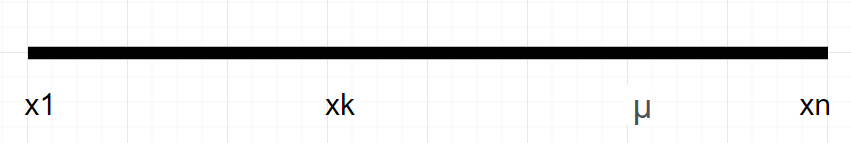
\includegraphics[width = \linewidth]{4.png}
\caption{Situation 4}
\end{figure}

Therefore, when $x_k$ = $x_1$ has the maximum value between $x_k$ and $\mu$. \\
As $F(\mu) = L_{\infty}(\mu,D) = |\mu - x_1| = \mu - x_1$ and $\mu$ is closer to $x_n$, when the distance between $\mu$ and $x_n$ is large enough but it does not exceed the distance between $\mu$ and $x_1$, $F(\mu)$ has the minimum value. That's when the distance between $\mu$ and $x_1$ is equal to the distance between $\mu$ and $x_n$, i.e. $\mu$ = $\frac{x_1 + x_n}{2}$.\\

Above all, the minimum value is $L_{\infty}$($\mu$, D) = $\frac{x_n - x_1}{2}$, when $\mu = \frac{x_1 + x_n}{2}$\\

Therefore, for the $L_{\infty}$ loss function, $L_{\infty}$($\mu$, D) = $max_{1\leq i\leq n}|\mu-x_i|$, show that the optimal choice for $\mu$ is $\frac{x_1+x_n}{2}$\\

4. \textbf{For the following data sets, compute the optimal representative µ with respect to the $L_2$, $L_1$ and $L_{\infty}$
loss function. Draw your result in a table as shown below. (You don’t need to show the calculations for
this.) Comment on how sensitive each loss function is to outliers.}

\begin{center}
\begin{tabular}{ |c|c|c|c|c|} 
\hline
$\mu$ & $L_1$ & $L_2$ & $L_{\infty}$\\
\hline
$\mathcal{D}_1$ & 2 & 2.2 & 2.5\\ 
$\mathcal{D}_2$ & 2 & 21.2 & 50\\ 
$\mathcal{D}_3$ & 30 & 35 & 50\\ 
\hline
\end{tabular}
\end{center}

$L_1$ is the least sensitive to the data because when $\mathcal{D}_2$ include 100 which includes a large outlier in the list, the result remains the same as the $\mathcal{D}_1$ which excludes any outlier in the list.\\
However,$L_{\infty}$ is the most sensitive to the data because when $\mathcal{D}_2$ include 100 which includes a large outlier in the list, the result obtained is more than 10 times that of other normal data. Even if the outlier is not obvious, it will produce results that deviate from the normal data\\
Talking to $L_2$, it is not sensitive when the outlier is not very far away from normal data. However, when the outlier is extremely far away from the normal data, it is sensitive and the result is more than 7 times that of other normal data.
\end{document}

